\chapter{2013}

\section*{一、选择题(本大题共 20 小题,每小题 2 分,共 40 分)}

1. 计算机算法指的是解决问题的有限运算序列, 它必须具备输入、输出和 (   )等 5 个特性。

A. 可执行性、可移植性和可扩充性

B. 可行性、确定性和有穷性

C. 确定性、有穷性和稳定性

D. 易读性、稳定性和安全性

2. 某算法代码段如下,其时间复杂度是(   )。

% 为了让字体和图片中的更像，并设置为C语言风格
\begin{lstlisting}[language=C, basicstyle=\ttfamily]
for(i=1; i<=n; ++i)
  for(j=1; j<=n; ++j)
    {     c[i][j]=0;
          for(k=1; k<=n; ++k)
            c[i][j]+=a[i][k]*b[k][j];
    }
\end{lstlisting}

A. \(O\left( {n}^{2}\right)\) B \(O\left( {n}^{3}\right)\) C. \(O\left( n\right)\) D. \(O\left( {n{\log }_{2}n}\right)\)

3. 和顺序(连续)存储结构相比,线性表的链式存储结构的优点是(   )。

A. 所有操作/运算的算法都简单 . B. 便于随机存取

C 便于插入和删除 D. 便于查找

4. 在某线性表中最常用的操作是在最后一个元素之后插入一个元素和删除第一个元素,则采用(   )存储方式最节省运算时间。

A. 单链表 

B. 仅有头指针的单循环链表

C. 双向链表 

D. 仅有尾指针的单循环链表

5. 在线性表的下列运算中,不会改变数据元素之间结构关系的运算是(   )。

A. 插入 B. 删除 C. 排序 D. 查找

6. 在解决计算机主机与打印机之间速度不匹配问题时通常设置一个打印数据缓冲区,主机将要输出的数据依次写入该缓冲区,而打印机则依次从该缓冲区中取出数据打印。则该缓冲区作为数据结构是一个(   )结构。

A. 队列 B. 栈

C. 链表 D. 都不是

7. 栈和队列的共同点有(   )。

A. 都是先进先出 B. 都是后进先出

C. 不会删除中间的元素 D. 完全没有共同点

8. 设循环队列中数组的下标范围是 0.. \(\mathrm{n} - 1\) ,其头指针 front 指向队首元素, rear 指向队尾元素,则队列的长度为 (  )。

A. rear-front 

B. rear-front +1

C. \(\left( {\text{ rear } - \text{ front } + 1}\right) \% \left( {\mathrm{n} + 1}\right)\) 

D. (rear-front \(+ \mathrm{n} + 1\) ) \%n

9. 数组 \(\mathrm{A}\) 中,每个元素 \(\mathrm{A}\) 的长度为 3 个字节,行下标 \(\mathrm{i}\) 从 1 到 8 ,列下标 \(\mathrm{j}\) 从 1 到 10 ,从首地址 SA 开始连续存放在存储器内,该数组按行优先存放时, 元素 \(\mathrm{A}\left\lbrack  8\right\rbrack  \left\lbrack  5\right\rbrack\) 的起始地址为(   )。

A. SA+141 B. SA+222

C. SA+144 D. SA+225

10. 二叉树中(树根为第 1 层)第 5 层上的结点个数最多为(   )

A. 8 B. 15 C. 16 D. 32

11. 高度为 3 的二叉平衡树(空树高度为 0 )最少有(   )个结点。

A. 4 B. 15 C. 11 D. 7

12. 设高度为 \(\mathrm{h}\) (空树高度为 0 ) 的二叉树上只有度为 0 和度为 2 的结点,则此类二叉树中所包含的结点数至少为(   )。

A. \(2\mathrm{\;h}\) B. \(2\mathrm{h} - 1\) C. \(2\mathrm{h} + 1\) D. h+1

13. 将一棵有 100 个结点的完全二叉树从上到下 (根这一层), 每一层上从左到右依次对结点进行编号, 根结点的编号为 1 , 则编号为 49 的结点的左孩子编号为(   )。

A. 98 B. 48 C. 99 D. 50

14. 一棵哈夫曼树(Huffman Tree)的 4 个叶子结点的权值分别为 3, 9, 2, 7, 该树的带权路径长度为(   )。

A 38 B. 37 C. 44 D. 46

15. 图的邻接矩阵表示法适用于表示 (   )。

A. 无向图 B. 有向图 C. 稠密图 D. 稀疏图

16. 设图连通 G 采用邻接表存储,则深度优先遍历算法的时间复杂度是(   )。

A. O(n) B. O(n+e) C. \(O\left( {n}^{2}\right)\) D. \(\mathrm{O}\left( {{\mathrm{n}}^{4}\mathrm{e}}\right)\)

17. 顺序查找算法在查找成功情况下的平均比较次数是(   )。

A. \({\mathrm{n}}\) B. \({\mathrm{n}}^{2}\) C. \(\log \left( \mathrm{n}\right)\) D \(\left( {n + 1}\right) /2\)

18. 散列 (哈希, Hash) 函数有一个共同性质, 即其函数取值在值域里呈现(   )。

A. 均匀分布 B. 正态分布 C. 泊松分布 D. 任意分布

19. 时间复杂度不受待排序序列初始状态的影响,总是 \(O\left( {n}^{2}\right)\) 的是(   )。

A. 直接插入排序 B. 快速排序 C. 简单选择排序 D. 归并排序


20. 以比较为基础的排序算法在最坏情况下的计算时间复杂度下界为(   )

A. \(O\left( {n}^{2}\right)\) B. \(O\left( {{\log }_{2}n}\right)\) C. \(O\left( n\right)\) D. \(O\left( {n{\log }_{2}n}\right)\)

\section*{二、填空题(本大题共 17 小题,每小题 2 分,共 34 分)}

1. 求整数 \(\mathrm{n}\left( {\mathrm{n} \geq  0}\right)\) 阶乘函数的递归算法如下,其时间复杂度是(   )

\begin{lstlisting}[language=C, basicstyle=\ttfamily]
long Factorial(long n) {
    if(n == 0) return 1;
    else return n*Factorial(n-1);
}
\end{lstlisting}

2. 某算法中的语句频度之和为 \(T\left( n\right)  = 2{n}^{2} + {5n} + 2\) ,则其时间复杂度为 (   )。

3. 已知栈的输入序列为 1,2,3,4,5,6,7输出序列为 a1, a2, a3, a4, a5, a6, a7 符合 a2 =7 条件的输出序列共有(   )个。

4. 采用特殊字符作为结尾的顺序存储方式存储,则串 “MyDataS” 最少需要 (   )个字符的存储空间。

5. 已知某二叉树的先序序列 ABCDEGF, 中序序列 CBEGDFA, 那么它的后序遍历序列是 (   )

6. 已知完全二叉树的第 4 层(根结点为第 1 层)总共只有 3 个结点,则其叶子结点数是(   )。

7. 某表达式二叉树按后序遍历的结果为 abcd-*+ef/-,令 \(a = 2,b = 3,c = 4,d = 5\) , \(e = 6,f = 2\) ,则该表达式的值等于(   )。

8. 在一棵度为 3 的树中, 度为 2 的结点个数是 1 , 度为 0 的结点个数是 6 , 则度为 3 的结点个数是(   )。

9. 高度为 \(\mathrm{k}\) (空树高度为 0 )的完全二叉树至少有(   )个结点。

10. 含 \(\mathrm{n}\) 个顶点的无向连通图中至少含有(   )条边。

11. 在具有 20 个元素的顺序表 (查找表) 上进行折半查找 (二分查找), 需比较五次并查找成功的元素个数是(   )

12. 判别下面的序列是否为堆(若是, 明确小根堆或大根堆)? (100,86,48,73,35,39,42,57,66,21);

13. 应用 Dijkstra's 算法(单源最短路径)求图 1 顶点 v6 到其他顶点的最短路径,最先求出的是顶点 \(\mathrm{v}6\) 到顶点(   )的最短路径。

14. 有 8 个球队参加的某联赛按单循环方式进行比赛,其需要进行的比赛场次为(   ), 和完全无向图的边数一样多。

15. 由 6 个权值构造的哈夫曼树(Huffman Tree)有(   )个结点。

16. 在非空 m 阶 B 树上。除根结点以外的所有其他内部结点含有(   )棵子树。

17. 给出图 2 的一个拓扑序列(   )。

% \begin{center}
% 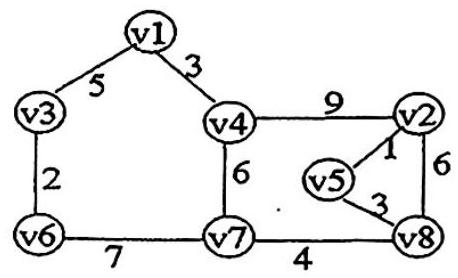
\includegraphics[width=0.3\textwidth]{images/2013/blank_17_1.jpg}
% 图 1
% \end{center}
% \hspace*{3em} 

\begin{figure}[htbp]
    \centering
    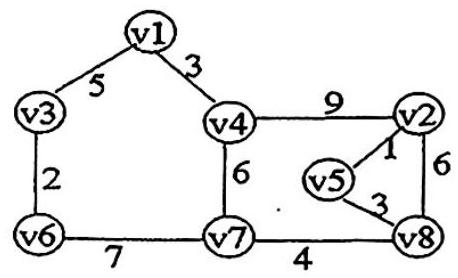
\includegraphics[width=0.3\textwidth]{images/2013/blank_17_1.jpg}
    \caption*{图1} % 使用带星号的 caption*
\end{figure}

\begin{figure}[htbp]
    \centering
    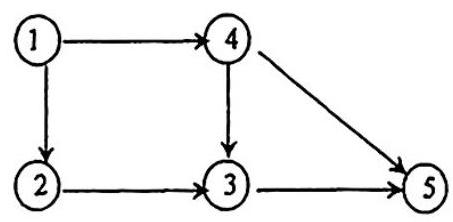
\includegraphics[width=0.3\textwidth]{images/2013/blank_17_2.jpg}
    \caption*{图2} % 使用带星号的 caption*
\end{figure}

\section*{三、问答题(本大题共 7 小题,每小题 8 分,共 56 分)}

1. 在一个长度为 \(\mathrm{n}\) 的单链表 \(\mathrm{L}\) 中,现需删除链表中 \(* \mathrm{p}\) 结点的前驱结点,试简要说明该操作的实现思想, 并分析时间复杂度。
\vspace{5em}

2. 具有 8 个结点的某森林的孩子一兄弟存储结构刚好构成完全二叉树。请画出原来的森林的结构。
\vspace{10em}

\newpage
3. 现有无向图如图 3 所示,从顶点 \(\mathrm{F}\) 开始使用 Prim(普里姆) 算法求图的最小生成树, 要求必须清楚地表明其生成过程。
\vspace{7em}

4. 现有无向图如图 3 所示, 完成下面任务: 

(1)画出图的邻接矩阵图示; 

(2)从顶点 \(\mathrm{H}\) 开始对图进行广度优先遍历,写出遍历结果。
\vspace{10em}

\newpage
5. 已知一棵二叉排序树结构如图 4 所示, 各结点的数据从小到大依次为 15,25,37,49,51,66,请重建出完整的原二叉树。
\vspace{10em}

6. 设 Hash 函数为 \(\mathrm{H}\left( \mathrm{{key}}\right)  = \mathrm{{key}}{\;\operatorname{mod}\;7}\) ,哈希表的地址空间为 \(0,1,\ldots ,{10}\) ,开始时哈希表为空, 用平方探测法解决冲突。回答下列问题:

1)请画出依次插入键值9,14,10,30,56后的哈希表？

2) 对表中关键字 14,30 和 56 进行查找时,所需进行的比较次数各为多少?
\vspace{10em}

\newpage
7. 对关键字序列(51,32,66,92,75,16,25,46)按从小到大进行快速排序。 设选第一个元素为支点/参考值 (pivot),写出排序过程中第 1 趟的划分结果；

\begin{figure}[htbp]
    \centering
    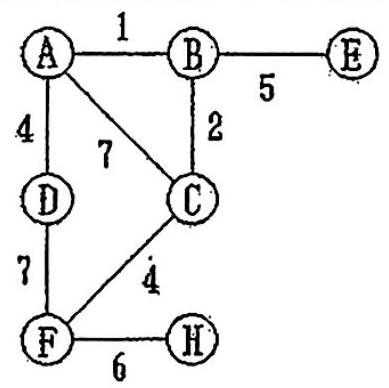
\includegraphics[width=0.3\textwidth]{images/2013/ask_7_1.jpg}
    \caption*{图3} % 使用带星号的 caption*
\end{figure}

\begin{figure}[htbp]
    \centering
    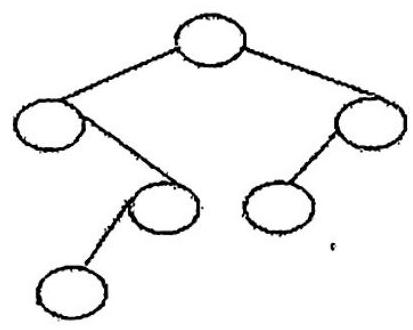
\includegraphics[width=0.3\textwidth]{images/2013/ask_7_2.jpg}
    \caption*{图4} % 使用带星号的 caption*
\end{figure}

\vspace{10em}

\section*{四、算法设计、分析题(本大题共 2 小题,每小题 10 分,共 20 分)}

1. 现有一棵二叉查找 (排序) 树 (Binary Search Tree) BST, 以二叉链表形式存储, 进行中序遍历可得到从小到大排列的有序序列。试设计一算法, 对该二叉查找树进行变换, 使得对新的二叉树进行中序遍历可得到从大到小排列的有序序列。要求:

(1)描述算法的基本设计思想。

(2)根据设计思想,描述算法的详细实现步骤 ,可使用伪代码、C或C++或 JAVA 语言,关键之处给出简要注释。

有关的数据结构已描述如下:

\begin{lstlisting}[language=C, basicstyle=\ttfamily]
struct Binary_node {
    int data;
    Binary_node *left;
    Binary_node *right;
}
\end{lstlisting}
\vspace{10em}

2. 某顺序表中的数据序列为降序序列, 试设计一算法将数据序列变换为升序序列。要求:

(1)描述算法的基本设计思想。

(2)根据设计思想,描述算法的详细实现步骤,可使用伪代码、C 或 C++或 JAVA 语言,关键之处给出简要注释。

(3)分析算法时间复杂度、空间复杂度。